\begin{task}{Timing Glitches}{}{}

  The Boolean algebra perspective on electronic circuits is a very powerful tool showing us that
  more or less every interesting functionality can be implemented by using only a single electronic
  building block (NAND). However, this perspective is incomplete. This task shows that the algebraic minimization
  of Boolean circuits can lead to so-called timing hazards or timing glitches and that real-world
  digital electronics might need to take into account these aspects.

  When turning from a input-output perspective as represented by a truth table to a timing perspective, one
  first defines a stimulus (often called testbench) which is a temporal trace of all input signal lines. A good
  stimulus consists of all states and all important transitions, at the moment, we will create only a stimulus
  for three bits which shows a problem.

  We follow an example from the given book \url{https://link-springer-com.eaccess.ub.tum.de/book/10.1007/978-3-030-13605-5}, which you can freely access. Try to follow this task before reading Chapter 4.5 in this book.

  Consider the following circuit:

  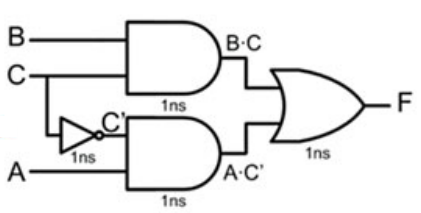
\includegraphics[width=.5\textwidth]{gfx/circuit_timingglitch.png}

  in which the timings are understood to be delays in the following sense: if a change on an input line implies
  a change to the output lines, then this change is performed 1ns later. 
  
  \begin{itemize}
  \item{Reconstruct the expression of this circuit}
  \item{Draw a Karnaugh map with A on the vertical axis and a Gray code for BC on the horizontal axis.}
  \item{Draw a time-signal diagram for 7ns with given signals $A =1$ and $B=1$ for all times. Signal $C$ starts
    as $C=1$ and changes to $C=0$ at t=2ns. Considering delays, derive the change of all signal lines in the circuit, namely, $BC$, $\overline{C} == C'$, $A\cdot \overline{C}$, and finally $F$.

    Explain all changes to signals at times.}

  \item{With the same stimulus as in the previous task, analyze the behaviour of the output of

    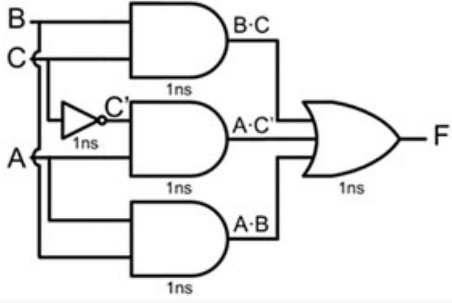
\includegraphics[width=.5\textwidth]{gfx/circuit_timingglitch_corrected.png}

  }
    

    \end{itemize}
  

\end{task}
